\chapter{Prototyping}
\begin{redbar}
Il \textbf{prototyping} è una fase fondamentale del processo di design nell'Interazione Uomo-Macchina (HCI). Rappresenta un'opportunità per esplorare e testare diverse soluzioni, valutare l'usabilità dell'interfaccia e raccogliere feedback dagli utenti prima di implementare il sistema finale. Il prototyping non riguarda solo la creazione di modelli fisici o digitali, ma serve anche come base per validare idee e ipotesi attraverso un processo iterativo.
\end{redbar}

Dopo aver creato uno storyboard per visualizzare i task principali che un utente deve eseguire, il passo successivo è immaginare l'interazione e progettare l'interfaccia utente (UI). Questo significa pensare non solo all'aspetto visivo, ma anche agli strumenti disponibili, come i dispositivi hardware, i widget e gli stili di interazione. È importante che la UI sia progettata considerando l'ecosistema in cui sarà utilizzata, tenendo conto di dove, quando e con chi l'interazione avverrà.

Tuttavia, è normale che il progetto iniziale non sia perfetto. Gli errori fanno parte del processo di design, e per questo è cruciale testare le idee con utenti reali. Questo permette di verificare se la UI è completa, comprensibile e facile da usare.

\section{Prototipo}
Un prototipo è un modello di un sistema interattivo che simula o anima alcuni aspetti o funzionalità del sistema finale, ma non tutti. Il prototipo permette ai progettisti di sperimentare la progettazione senza sviluppare l'intero sistema. Può essere utilizzato per testare concetti e idee in un ambiente controllato e per raccogliere feedback prima della fase di sviluppo completa. Un esempio di prototipo potrebbe essere un mockup di uno smartphone, in cui vengono simulate solo alcune funzionalità, come la navigazione tra le schermate o l’interazione con i widget.

Esistono diversi modi di utilizzare i prototipi. In generale, essi vengono impiegati per:
\begin{itemize}
    \item Provare e validare un'idea o un concetto: ad esempio, testare un nuovo sistema di navigazione per un'app.
    \item Imparare dagli utenti: raccogliere feedback diretto per migliorare il design.
    \item Sperimentare versioni intermedie o finali: i prototipi permettono di vedere come si evolve l'interazione con il sistema man mano che si aggiungono nuove funzionalità.
\end{itemize}

Esistono tre approcci principali al prototyping:
\begin{enumerate}
    \item \textit{Prototyping “throw away”:} Il prototipo viene creato per esplorare un'idea, e una volta ottenute le informazioni necessarie, viene scartato.
    \item \textit{Prototyping incrementale:} Le varie funzioni vengono aggiunte una alla volta al prototipo, permettendo di testare l'interfaccia in modo progressivo.
    \item \textit{Prototyping evolutivo:} Ogni nuovo prototipo si basa su quello precedente, migliorando gradualmente le funzionalità e il design.
\end{enumerate}

\section{Ciclo di prototypazione}
Il design delle interfacce è raramente perfetto al primo tentativo. È fondamentale seguire un ciclo iterativo che prevede la creazione di un prototipo, la sua validazione con utenti reali e, in base ai risultati, la riprogettazione dell'interfaccia. Questo processo continua fino a ottenere un sistema che soddisfi le esigenze degli utenti. Il ciclo di prototyping segue una sequenza di progettazione, test e revisione.

Durante il processo di prototipazione iterativa, è utile utilizzare il concetto di hill climbing, che si riferisce al miglioramento continuo del progetto. Ogni iterazione del prototipo cerca di superare i difetti individuati nella versione precedente, migliorando gradualmente il design. Questo processo funziona solo se si riesce a capire a fondo cosa è sbagliato nel progetto e si propongono soluzioni mirate.

Uno dei problemi principali nel prototyping è il tempo necessario per realizzare i prototipi. Creare un prototipo richiede tempo, e se questo viene scartato, può sembrare tempo sprecato. Tuttavia, il prototyping rapido può aiutare a ridurre questa sensazione, purché non si sacrifichi la qualità del processo di valutazione.
Un'altra sfida è la pianificazione. Poiché il processo di prototyping può essere imprevedibile, è difficile stabilire tempi e costi precisi. Spesso, il committente e il progettista devono negoziare continuamente per mantenere il progetto in linea con il budget.
Infine, i prototipi possono trascurare alcune caratteristiche non funzionali, come la sicurezza, l'affidabilità o il tempo di risposta. Questi aspetti, se ignorati durante il prototyping, possono creare problemi nella fase di sviluppo finale.

Un ultimo problema da tenere presente è l'inerzia del design. Una volta presa una decisione progettuale, c'è il rischio che questa non venga mai più rivista, anche se si rivela errata. Il processo iterativo di prototipazione deve quindi includere una revisione costante delle scelte iniziali, per evitare di costruire l'interfaccia su fondamenta sbagliate. È essenziale individuare e affrontare le cause profonde dei problemi, piuttosto che limitarsi a correggere i sintomi.

Uno degli errori comuni durante il prototyping è focalizzarsi troppo presto sull’interfaccia utente (UI) senza aver prima compreso a fondo il task che l'utente deve completare. È importante quindi iniziare comprendendo bene i compiti e i bisogni dell’utente, per poi costruire la UI attorno a questi.

Esistono diverse tecniche di prototyping. Ogni tecnica ha vantaggi specifici a seconda del contesto in cui viene utilizzata e degli obiettivi del team di design.

\section{Low fidelity prototypes}
I low fidelity prototypes sono utilizzati nelle prime fasi del processo di progettazione. Si tratta spesso di modelli realizzati su carta, come i mock-up disegnati a mano, che possono includere più fogli di diverse dimensioni per rappresentare vari stati dell’interfaccia. Questi prototipi sono strumenti rapidi per esplorare le prime idee e testare l’interazione utente, consentendo di individuare e risolvere problemi di design senza investire troppo tempo o risorse.

\subsection{Paper prototypes}
Un tipo di low fidelity prototypes è il paper prototype, dove un’interfaccia disegnata a mano simula l’aspetto visivo di un’app. Le diverse schermate e gli elementi interattivi (come finestre, menu o dialog box) possono essere rappresentati da pezzi di carta che vengono posizionati e manipolati manualmente, simulando un’interazione reale. Ad esempio, un dito che tocca uno schermo simulato equivale a un clic del mouse, e la scrittura su un pezzo di carta rappresenta l'inserimento di testo. Una persona funge da "computer", simulando le risposte del sistema, come aggiornamenti di finestre o feedback, interagendo con i vari pezzi di carta. Questo tipo di prototipo, sebbene a bassa fedeltà in termini di aspetto visivo, può raggiungere un'elevata fedeltà nella simulazione delle interazioni e del flusso di lavoro.

Il paper prototyping richiede pochi materiali di base: carta, fogli trasparenti, penne, pennarelli, post-it, forbici e nastro adesivo. Questi strumenti semplici permettono di costruire prototipi in modo rapido ed economico, favorendo la sperimentazione continua. Utilizzando stencil per elementi dell’interfaccia utente (UI) o stampando schermate già esistenti, è possibile creare componenti riutilizzabili che velocizzano ulteriormente il processo.

\begin{figure}[ht]
    \centering
    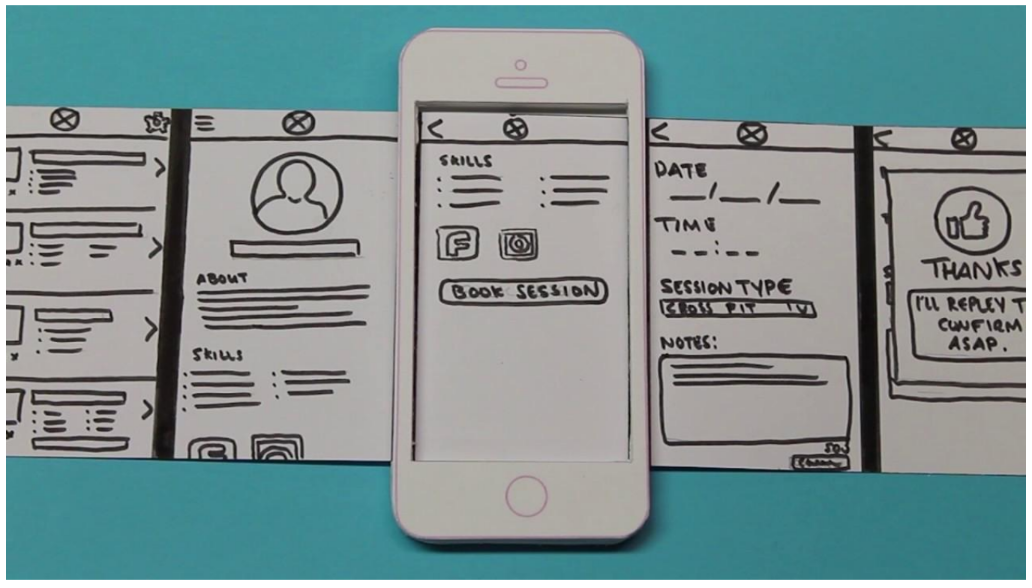
\includegraphics[width=0.6\linewidth]{images/paper-prototype.PNG}
    \caption{Esempio di paper prototype}
    \label{fig:paper-prototype}
\end{figure}

Il principale vantaggio del paper prototyping è la sua rapidità. Schizzare su carta è molto più veloce che programmare, e modificare il design tra un test e l'altro è altrettanto semplice. 
Il prototyping su carta permette di concentrarsi sugli aspetti più importanti del design, senza perdersi nei dettagli tecnici. Gli utenti e i clienti possono partecipare attivamente alla discussione, fornendo feedback creativi e non limitati a questioni estetiche o funzionali minori. Questo approccio rende il paper prototyping accessibile anche ai non programmatori, dato che richiede solo abilità di base.

Durante il test di un paper prototype, il team di progettazione assume vari ruoli. Un membro del team funge da computer, simulando il comportamento del sistema, ma senza fornire feedback. Il facilitatore presenta l'interfaccia e i task all'utente, incoraggiandolo a pensare ad alta voce e descrivere le proprie azioni e pensieri mentre interagisce con il prototipo. L'osservatore si limita a prendere appunti senza intervenire, annotando dettagli importanti come le reazioni dell'utente, le difficoltà incontrate o i suggerimenti spontanei.

Il testing dei paper prototypes consente di raccogliere informazioni importanti. Ad esempio, permette di valutare se gli utenti comprendono il modello concettuale dell'interfaccia e se la funzionalità proposta soddisfa i loro bisogni. Il test rivela anche quanto sia intuitiva la navigazione, se gli utenti riescono a orientarsi facilmente tra le varie schermate e se la terminologia utilizzata è chiara. Inoltre, è possibile valutare i contenuti visivi delle schermate, identificando quali informazioni devono essere presenti per garantire un'interazione fluida.

Tuttavia, ci sono anche dei limiti. Con un paper prototype non è possibile testare aspetti come i colori, i font, il layout o l'efficienza dell’interfaccia. Inoltre, gli utenti tendono a essere più deliberati e meno esplorativi quando interagiscono con un prototipo di carta, sapendo che stanno lavorando con un modello non finito.

\section{Medium fidelity prototypes}
I prototipi a media fedeltà rappresentano una fase avanzata del processo di progettazione rispetto ai prototipi su carta, poiché offrono una visione più dettagliata dell'interfaccia e del layout. Tuttavia, non raggiungono la completezza dei prototipi ad alta fedeltà in termini di comportamento e interattività. Sono particolarmente utili per simulare l'interazione dell'utente con il sistema, testando la navigazione tra le schermate e il flusso generale senza concentrarsi su aspetti grafici o estetici.

Questi prototipi vengono realizzati tramite software interattivi che simulano l'aspetto di un'interfaccia utente, accettano alcuni input e rispondono agli utenti passando da una schermata all'altra. Sono spesso definiti mockup o wireframe interattivi, poiché rappresentano una versione semplificata dell’interfaccia.

La grafica nei prototipi a media fedeltà è stilizzata e spesso in bianco e nero o in scala di grigi, con l’intento di trasmettere l’impressione che il design sia ancora in fase preliminare. Ciò permette agli utenti e ai designer di concentrarsi sugli aspetti funzionali e strutturali del sistema, senza distrarsi con dettagli estetici come i colori o i font.

Un aspetto importante nello sviluppo di prototipi a media fedeltà è l'uso di librerie di design per interfacce utente (UI). Queste librerie forniscono una serie di componenti predefiniti e riutilizzabili, come pulsanti, menu e barre di navigazione, che semplificano la creazione di mockup interattivi. Le librerie aiutano a mantenere una coerenza visiva e di interazione tra le varie schermate, rendendo più facile e veloce la progettazione del prototipo.

\begin{figure}[ht]
    \centering
    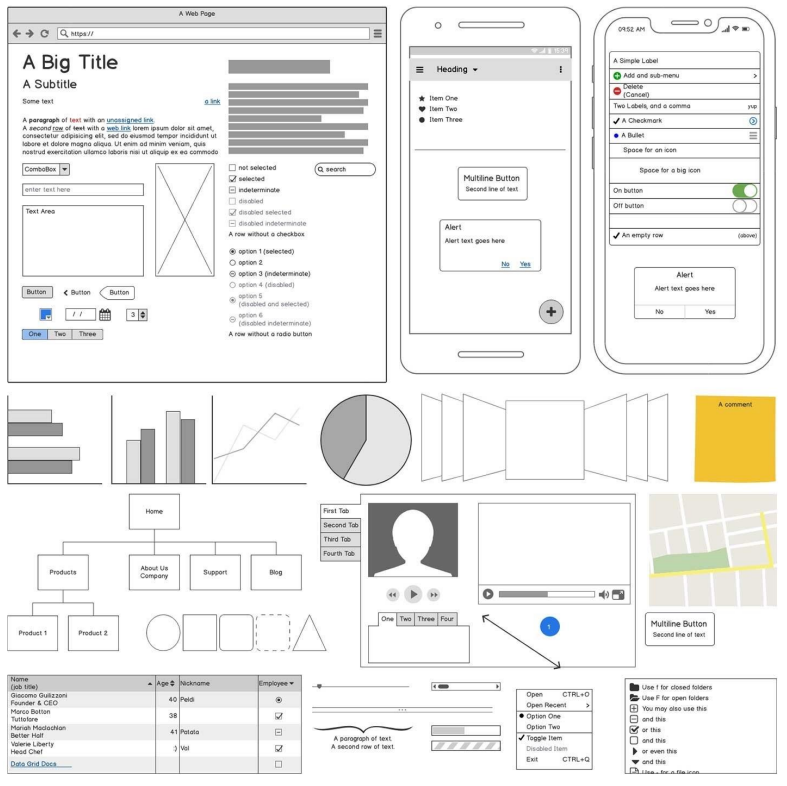
\includegraphics[width=0.7\linewidth]{images/medium-fidelity-prototype.PNG}
    \caption{Medium fidelity prototype}
    \label{fig:medium-fidelity-prototype}
\end{figure}

Esistono diversi strumenti utili per creare prototipi a media fedeltà. Tra i più popolari troviamo Balsamiq, un tool che offre un'interfaccia semplice e intuitiva per la creazione di wireframe interattivi. Moqups e Figma sono altre opzioni comunemente utilizzate.
Questi strumenti permettono di progettare interfacce navigabili, in cui l'utente può cliccare su vari elementi per passare da una schermata all'altra. Tuttavia, le interazioni nei prototipi a media fedeltà sono ancora limitate: gli utenti possono cliccare sui pulsanti e navigare tra le pagine, ma non possono inserire dati o eseguire operazioni complesse.
Questo può portare a una sorta di “caccia al punto cliccabile”, in cui gli utenti cercano i pochi elementi attivi che consentono di navigare tra le schermate.

Per questi motivi, i prototipi a media fedeltà sono ottimi per testare la comprensione dell'interfaccia e il flusso di navigazione, ma non sono adatti a valutare il comportamento dinamico del sistema.

\section{High fidelity prototypes}
I prototipi ad alta fedeltà rappresentano la versione più avanzata e dettagliata di un'interfaccia. Questi prototipi assomigliano in tutto e per tutto al prodotto finale, con un layout, colori, e grafica che corrispondono all'aspetto reale del sistema.

I prototipi ad alta fedeltà sono realizzati utilizzando strumenti di progettazione che permettono di creare interfacce realistiche con widget funzionanti e comportamenti interattivi verosimili. La differenza principale tra un prototipo ad alta fedeltà e un'applicazione completa sta nel fatto che il prototipo è progettato per simulare le interazioni, ma non sempre include l'intero backend, cioè la logica complessa o le interazioni con il database.

Il vantaggio di questo approccio è che l'interfaccia può essere testata in un contesto che sembra reale, offrendo agli utenti l'opportunità di esplorare l'interfaccia e di dare feedback sul layout, sui colori e sull'organizzazione visiva. Tuttavia, un rischio è che, poiché il prototipo appare “completo”, gli utenti potrebbero focalizzarsi su dettagli estetici piuttosto che sugli aspetti funzionali e interattivi. Ad esempio, potrebbero concentrarsi troppo sui colori, sui font o sulla grafica piuttosto che sul fatto che l’interfaccia risponda efficacemente ai loro bisogni.

Uno degli aspetti che si possono valutare con i prototipi ad alta fedeltà è il layout delle schermate. Questo permette di capire se gli utenti trovano le informazioni importanti con facilità o se l'interfaccia risulta eccessivamente complessa o disordinata.

\begin{figure}[ht]
    \centering
    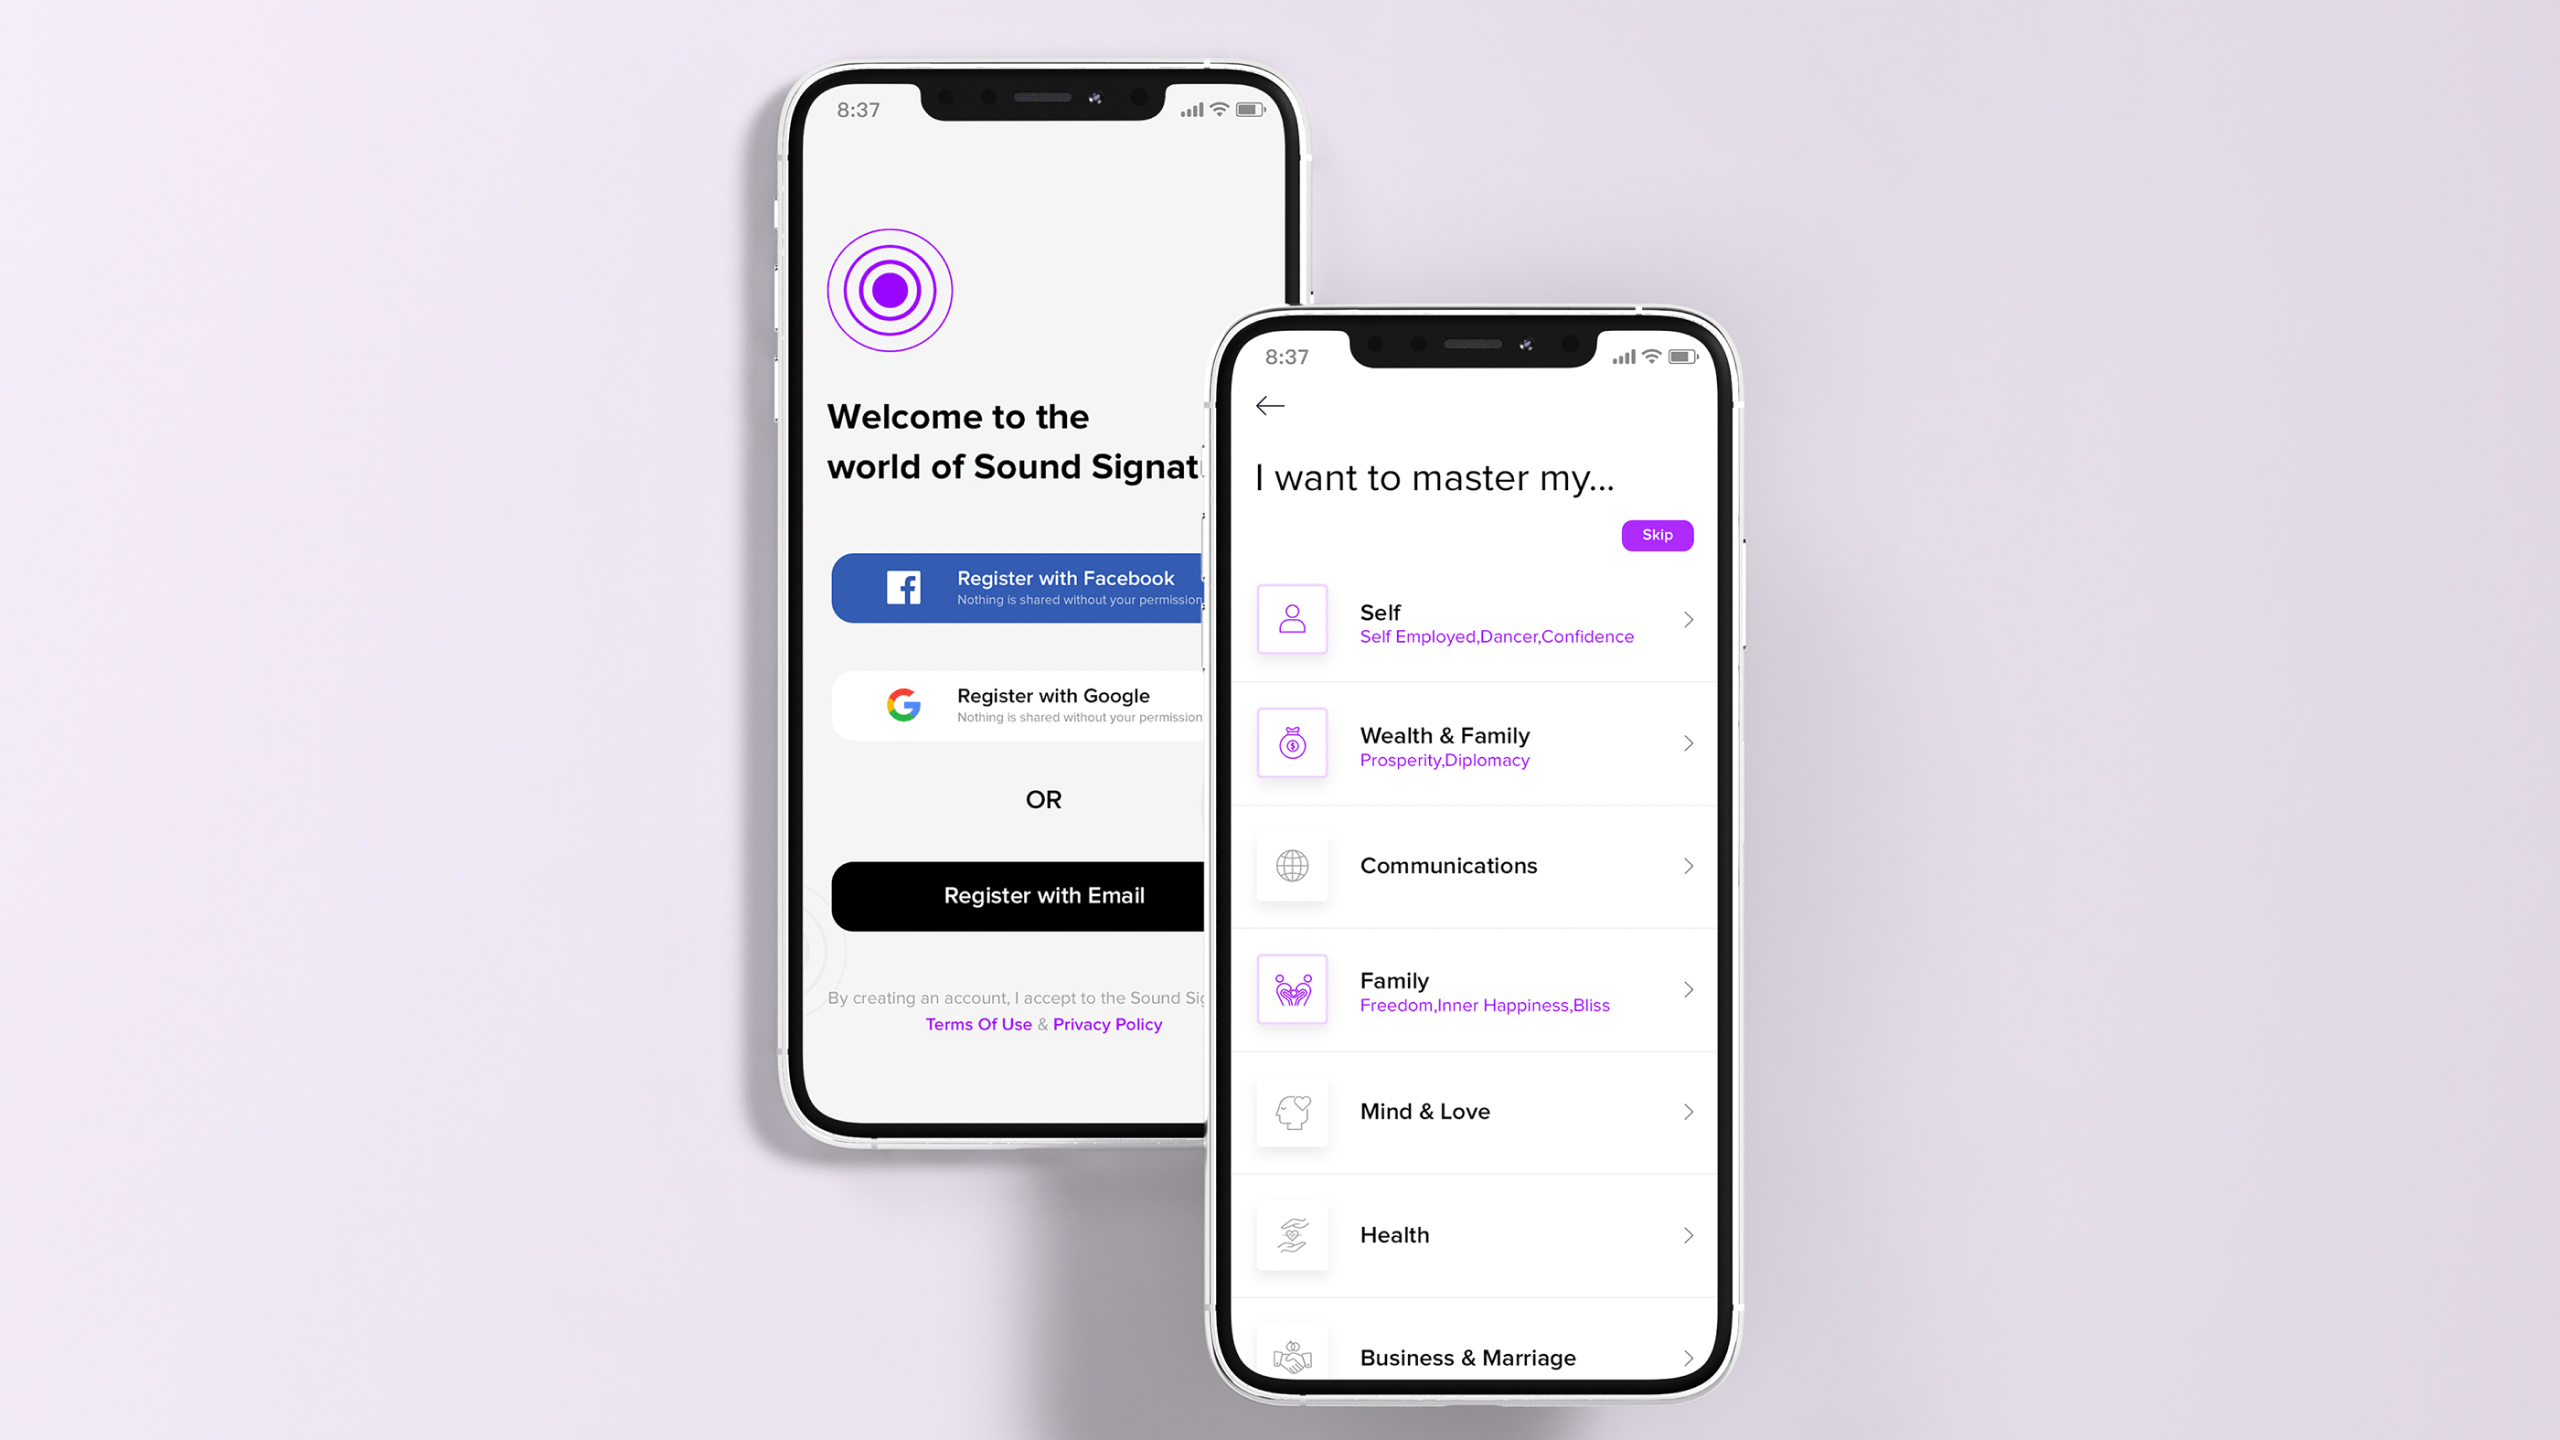
\includegraphics[width=0.6\linewidth]{images/high-fidelity-prototype.jpg}
    \caption{High fidelity prototype}
    \label{fig:high-fidelity-prototype}
\end{figure}

Un altro elemento che può essere valutato riguarda colori, font e icone. Questi elementi visivi sono cruciali per la user experience (UX) e per la percezione dell'interfaccia da parte dell'utente. Anche il feedback interattivo può essere testato: ci si può chiedere se gli utenti notano e rispondono correttamente ai messaggi della barra di stato, ai cambiamenti di cursore o ad altri segnali visivi che indicano l'avanzamento delle operazioni.

I problemi di efficienza sono un'altra area di valutazione. Ad esempio, si può osservare se i controlli sono abbastanza grandi da essere cliccati comodamente, se gli elementi interattivi sono disposti in modo logico o se liste di scorrimento troppo lunghe creano frustrazione. In breve, un prototipo ad alta fedeltà consente di esaminare dettagli molto specifici della UI, che possono avere un impatto importante sull'esperienza utente complessiva.

Esistono diversi strumenti per la creazione di prototipi ad alta fedeltà. Tra i più popolari vi sono InVision e Figma, che permettono di creare interfacce altamente interattive e realistiche. Questi strumenti permettono di creare prototipi senza scrivere codice, rendendo possibile la creazione di layout e interfacce completamente funzionanti.

\subsection{Metodo "Wizard of Oz"}
Una tecnica particolare per simulare tecnologie non ancora completamente implementate è il Wizard of Oz. Questo approccio consente di testare un'applicazione che sembra completa, con interfaccia e algoritmi finalizzati, ma senza dover scrivere tutto il codice necessario. Un essere umano simula il comportamento del sistema, controllando l'interfaccia dietro le quinte, come un mago nascosto dietro un sipario. Questo metodo viene spesso utilizzato per testare applicazioni che utilizzano tecnologie complesse o non ancora pronte, come il riconoscimento vocale o l’intelligenza artificiale.

Per implementare questa tecnica, è necessario scegliere task specifici da simulare, creando mock-up dell'interfaccia che consentano al "mago" di intervenire nei punti critici. Un esempio pratico potrebbe riguardare lo sviluppo di un’app di assistente virtuale, dove il sistema di riconoscimento vocale non è ancora implementato. Il mago, nascosto dietro il sistema, risponde manualmente alle richieste dell’utente, simulando l'algoritmo di risposta automatica.

Questo approccio ha diversi vantaggi. Innanzitutto, è più veloce e meno costoso rispetto allo sviluppo di un prototipo completamente interattivo. Inoltre, consente di creare diverse varianti del prototipo in tempi rapidi, testando scenari che sarebbero difficili da implementare con un codice reale. Il "mago" può anche aiutare a identificare bug o problemi di design, fornendo al team di progettazione una comprensione più dettagliata di come dovrebbero funzionare gli algoritmi finali.

Nonostante i vantaggi, il metodo Wizard of Oz presenta alcuni rischi. La simulazione manuale può portare a ottimismo eccessivo riguardo alle capacità future del sistema. Ad esempio, un sistema di riconoscimento vocale simulato dal mago potrebbe funzionare senza errori, mentre un sistema reale potrebbe avere tassi di errore significativi. Inoltre, il comportamento del mago è difficile da replicare esattamente come farebbe una macchina, e potrebbe rispondere in modo più efficiente di quanto un sistema reale riuscirebbe a fare.